\section{Project 3 - Filtering in Frequency Domain}

\subsection{Project Proposal}
Implement the ideal, Butterworth and Gaussian lowpass and highpass filters and the results under different parameters using the image character\_test\_pattern.tif

\subsection{Preliminaries}
\subsubsection{Summary of Fourier transform properties}

\begin{table}[h]
	\caption{Summary of useful formulas.}
	\centering
	\begin{tabular}{|l|m{0.6\columnwidth}|}\hline
		Name & Expression(s) \\ \hline
		1D FT & \begin{equation}F(u)=\int_{-\infty}^\infty f(t)e^{-j2 \pi ut}dt \end{equation} \\ 
		1D IFT & \begin{equation}f(t)=\int_{-\infty}^\infty F(u)e^{j2 \pi ut}du\end{equation} \\
		1D DFT & \begin{equation}F(u)=\sum_{t=0}^{M-1}f(t)e^{-j2\pi ut/M} \end{equation} \\
		1D IDFT & \begin{equation}f(t)=\frac{1}{M}\sum_{u=0}^{M-1}F(u)e^{j2\pi ut/M}\end{equation} \\
		2D FT & \begin{equation} F(u,v)=\int_{-\infty}^\infty \int_{-\infty}^\infty f(x,y)e^{-j2 \pi (ux+vy)}dxdy \end{equation} \\
		2D DFT & \begin{equation} F(u,v)= \sum_{x=0}^{M-1}\sum_{y=0}^{N-1} f(x,y)e^{-j2\pi (ux/M+vy/N)}\end{equation} \\
		2D IDFT & \begin{equation} f(x,y) = \frac{1}{MN}\sum_{u=0}^{M-1}\sum_{v=0}^{N-1]}F(u,v)e^{j2\pi(ux/M+vy/N)} \end{equation} \\
		Power spectrum & \begin{equation} P(u,v)=|F(u,v)|^2 \end{equation} \\
		\hline
	\end{tabular}
\end{table}

\subsubsection{Steps for filtering in the frequency domain}
\begin{enumerate}
	\item Given an input image $f(x,y)$ of size $M\times N$, obtain the padding parameters $P=2M$ and $Q=2N$.Form a padded image, $f_p(x,y)$, of size $P\times Q$ by appending zeros.
	\item Multiply $f_p(x,y)$ by $(-1)^{x+y}$ to center its transform.
	\item Compute the DFT, $F(u,v)$ of the image from centered padded image.
	\item Generate a real, symmetric filter function $H(u,v)$ of size $P \times Q$ with center at coordinates $(P/2, Q/2)$. Form the product $G(u,v)=H(u,v)F(u,v)$.
	\item Obtain the precessed image: $g_p(x,y)=\left\{ \text{real}\left[\ \mathcal{F}^{-1}[G(u,v)] \right] \right\}(-1)^{x+y}$ where the real part is selected in order to ignore parasitic complex components resulting from computational inaccuracies.
	\item Obtain the final processed result, $g(x,y)$, by extracting the top left $M\times N$ quadrant of $g_p(x,y)$
\end{enumerate}


\subsection{Frequency Domain Filters}
The filters used here all involving $D(u,v)$, which is the distance between $(u,v)$ in frequency domain and the center of the frequency rectangle \begin{equation} D(u,v) = \left[ (u-P/2)^2+(v-Q/2)^2 \right]^{1/2} \end{equation}. The 'pass' disappears in word 'lowpass' and 'highpass' means we set a range for the things reserved. The range is expressed as a value $D_0$ of $D(u,v)$. The percentage of power enclosed by the circle of radius $D_0$ with origin at the center of the frequency rectangle is \begin{equation} \alpha=100\left[\ \sum_u\sum_vP(u,v)/P_T \right] ~~~~ \text{(u,v) is inside the circle}\end{equation}
The three kind of frequency domain filters used in this project are \emph{ideal filter}, \emph{Butterworth filter} and \emph{Gaussian filter}. Their lowpass version and highpass version are in Table.\ref{table:3filters}. \\

\begin{table}[h]
	\caption{Summary of 3 filters.}
	\label{table:3filters}
	\centering
	\begin{tabular}{|l|m{0.6\columnwidth}|}
	\hline
		Name & Expression(s) \\ \hline
		Ideal lowpass filter (ILPF) & 
		\begin{equation} H(u,v) = \left \{ \begin{array}{rcl}
								1 & \text{if $D(u,v)\leq D_0$} \\
								0 & \text{otherwise}  \end{array} \right.
 		\end{equation} \\ \hline
		Butterworth lowpass filter (BLPF) & \begin{equation} H(u,v)=\frac{1}{1+[D(u,v)/D_0]^{2n}} \end{equation} \\ \hline
		Gaussian lowpass filter (GLPF) & \begin{equation} H(u,v)=e^{-D^2(u,v)/2D_0^2} \end{equation} \\ 
	\hline
		Ideal highpass filter (IHPF) & 
		\begin{equation} H(u,v) = \left \{ \begin{array}{rcl}
								0 & \text{if $D(u,v)\leq D_0$} \\
								1 & \text{otherwise}  \end{array} \right.
 		\end{equation} \\ \hline
		Butterworth highpass filter (BHPF) & \begin{equation} H(u,v)=\frac{1}{1+[D_0/D(u,v)]^{2n}} \end{equation} \\ \hline
		Gaussian highpass filter (GHPF) & \begin{equation} H(u,v)=1-e^{-D^2(u,v)/2D_0^2} \end{equation} \\ 
	\hline
	\end{tabular}
\end{table}

\subsection{Experiment}
The original test image of size $688 \times 688$ pixels and its non-padded centered Fourier spectrum are in Figure.\ref{fig:origin3}.
\begin{figure}[h!]
	\centering
	\begin{subfigure}[b]{0.45\linewidth}
		
\includegraphics[width=\linewidth]{myfigure/p3/characters_test_pattern.png}
		\caption{}
		\label{fig:orig}
	\end{subfigure}
  	\begin{subfigure}[b]{0.45\linewidth}
		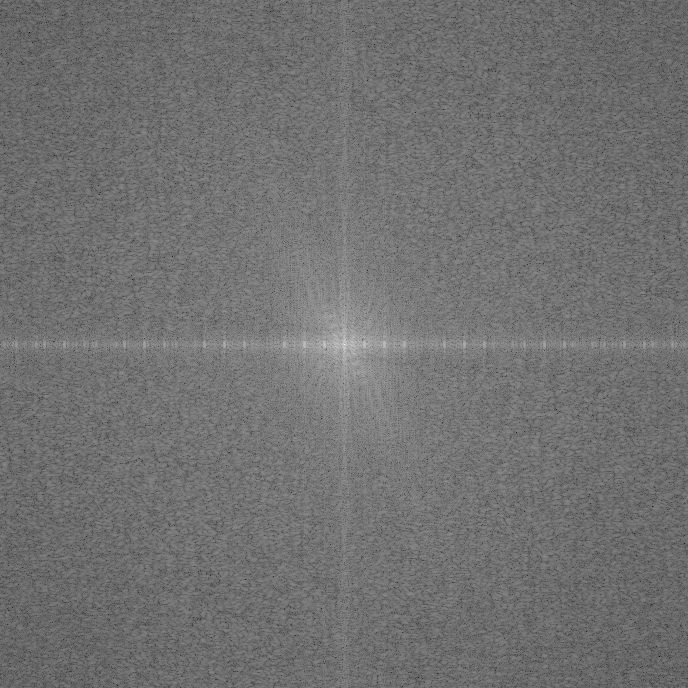
\includegraphics[width=\linewidth]{myfigure/p3/spectrum.png}
		\caption{}
		\label{fig:spectrum}
	\end{subfigure}
  	\caption{(\ref{fig:orig})Original test image of size $688\times 688$ pixels. (\ref{fig:spectrum})Non-padded centered Fourier spectrum of the original test image.}
  	\label{fig:origin3}
\end{figure}


\subsubsection{Image smoothing by lowpass filtering}
Edges and other sharp intensity transitions (such as noise) in an image contribute significantly to the high frequency content of its Fourier transform. Hence, smoothing (blurring) is achieved in the frequency domain by high-frequency attenuation; that is, by lowpass filtering. \\

I use 4 values of $D_0$ (10, 100, 1000, 4000) as the parameter of lowpass filters, generate the smoothed images and calculate power ratio of the filtering. The result is displayed in Figure.\ref{fig:ILPF}, Figure.\ref{fig:BLPF} and Figure.\ref{fig:GLPF}. In Butterworth filtering, I use $n=2$ as the order. 

\begin{figure}[h!]
	\centering
	\begin{subfigure}[b]{0.45\linewidth}
		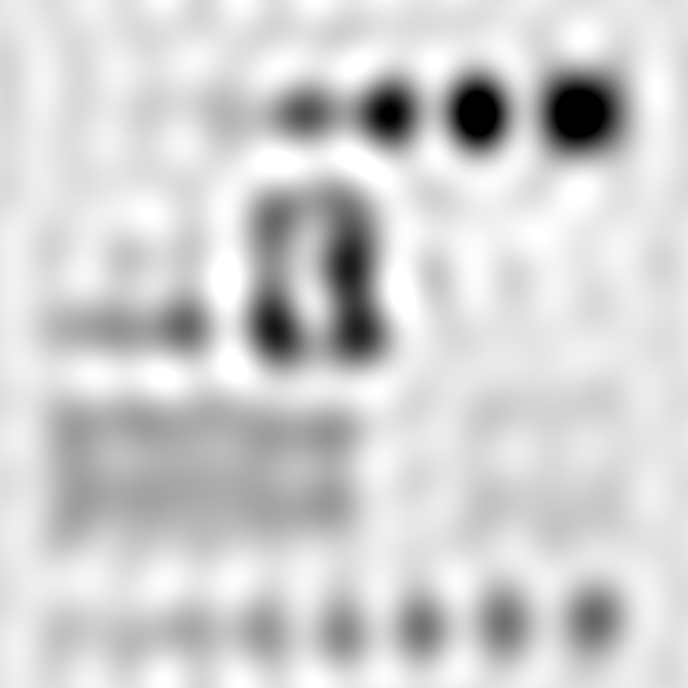
\includegraphics[width=\linewidth]{myfigure/p3/ILPF_10.png}
		\caption{$D_0=10$, power ratio=0.9098}
		\label{fig:ILPF_10}
	\end{subfigure}
  	\begin{subfigure}[b]{0.45\linewidth}
		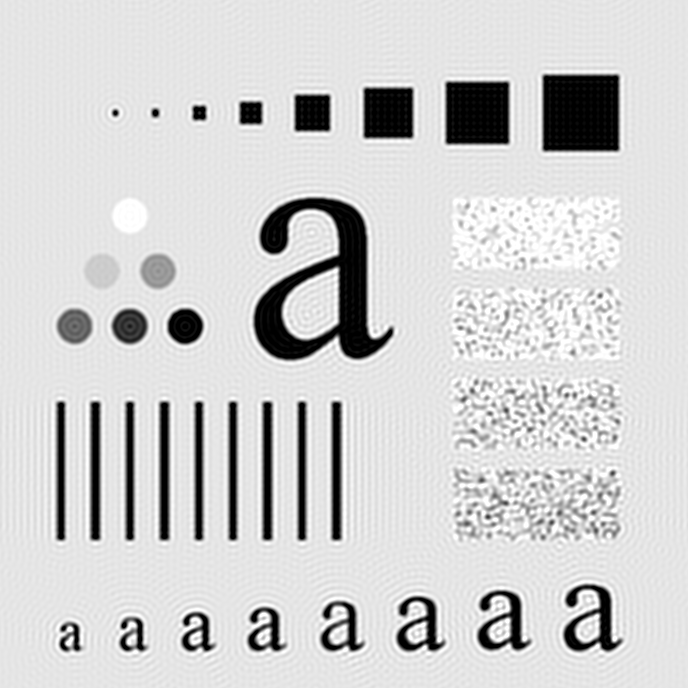
\includegraphics[width=\linewidth]{myfigure/p3/ILPF_100.png}
		\caption{$D_0=100$, power ratio=0.9231}
		\label{fig:ILPF_100}
	\end{subfigure}
	\begin{subfigure}[b]{0.45\linewidth}
		
\includegraphics[width=\linewidth]{myfigure/p3/ILPF_1000.png}
		\caption{$D_0=1000$, power ratio=0.9971}
		\label{fig:ILPF_1000}
	\end{subfigure}
  	\begin{subfigure}[b]{0.45\linewidth}
		
\includegraphics[width=\linewidth]{myfigure/p3/ILPF_4000.png}
		\caption{$D_0=4000$, power ratio=1.0000}
		\label{fig:ILPF_4000}
	\end{subfigure}
  	\caption{Results of ideal lowpass filtering.}
  	\label{fig:ILPF}
\end{figure}

\begin{figure}[h!]
	\centering
	\begin{subfigure}[b]{0.45\linewidth}
		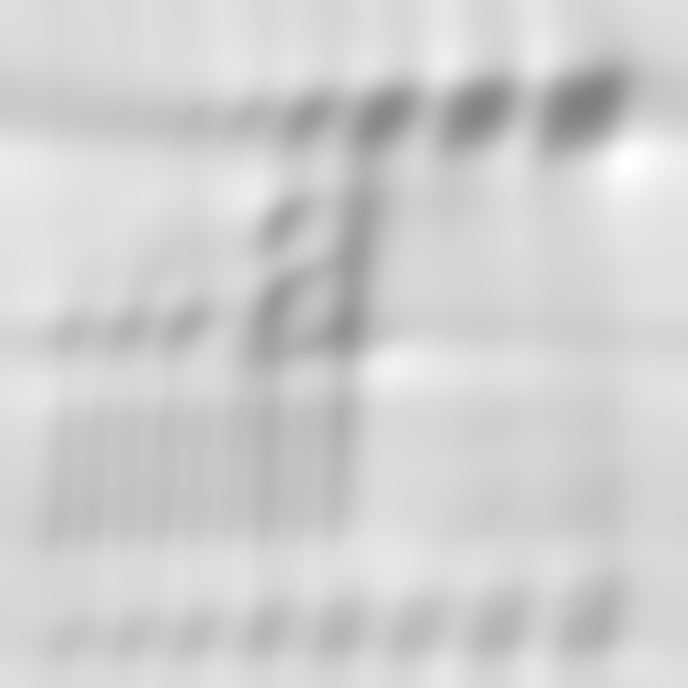
\includegraphics[width=\linewidth]{myfigure/p3/BLPF_10.png}
		\caption{$D_0=10$, power ratio=0.9076}
		\label{fig:BLPF_10}
	\end{subfigure}
  	\begin{subfigure}[b]{0.45\linewidth}
		
\includegraphics[width=\linewidth]{myfigure/p3/BLPF_100.png}
		\caption{$D_0=100$, power ratio=0.9223}
		\label{fig:BLPF_100}
	\end{subfigure}
	\begin{subfigure}[b]{0.45\linewidth}
		
\includegraphics[width=\linewidth]{myfigure/p3/BLPF_1000.png}
		\caption{$D_0=1000$, power ratio=0.9673}
		\label{fig:BLPF_1000}
	\end{subfigure}
  	\begin{subfigure}[b]{0.45\linewidth}
		
\includegraphics[width=\linewidth]{myfigure/p3/BLPF_4000.png}
		\caption{$D_0=4000$, power ratio=0.9997}
		\label{fig:BLPF_4000}
	\end{subfigure}
  	\caption{Results of Butterworth lowpass filtering.}
  	\label{fig:BLPF}
\end{figure}

\begin{figure}[h!]
	\centering
	\begin{subfigure}[b]{0.45\linewidth}
		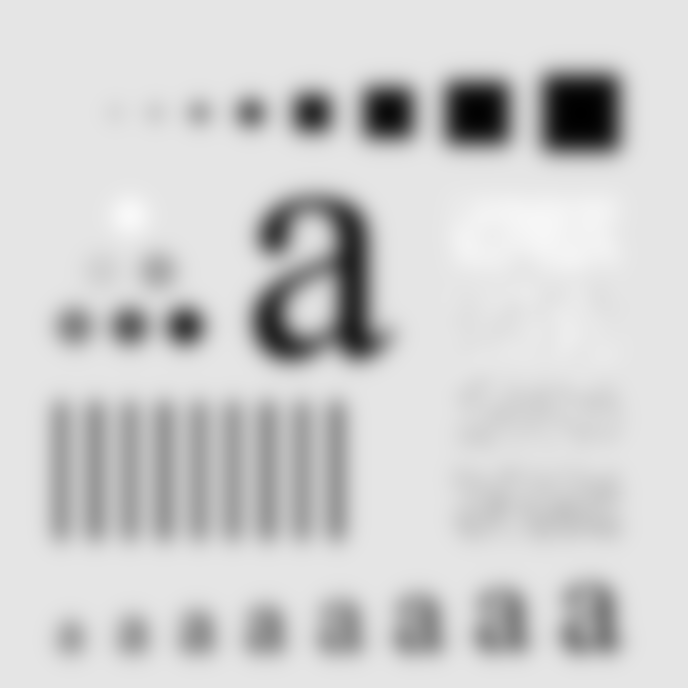
\includegraphics[width=\linewidth]{myfigure/p3/GLPF_10.png}
		\caption{$D_0=10$, power ratio=0.0.9075}
		\label{fig:GLPF_10}
	\end{subfigure}
  	\begin{subfigure}[b]{0.45\linewidth}
		
\includegraphics[width=\linewidth]{myfigure/p3/GLPF_100.png}
		\caption{$D_0=100$, power ratio=0.9219}
		\label{fig:GLPF_100}
	\end{subfigure}
	\begin{subfigure}[b]{0.45\linewidth}
		
\includegraphics[width=\linewidth]{myfigure/p3/GLPF_1000.png}
		\caption{$D_0=1000$, power ratio=0.9673}
		\label{fig:GLPF_1000}
	\end{subfigure}
  	\begin{subfigure}[b]{0.45\linewidth}
		
\includegraphics[width=\linewidth]{myfigure/p3/GLPF_4000.png}
		\caption{$D_0=4000$, power ratio=0.9972}
		\label{fig:GLPF_4000}
	\end{subfigure}
  	\caption{Results of Gaussian lowpass filtering.}
  	\label{fig:GLPF}
\end{figure}


\subsubsection{Image sharpening by highpass filtering}
Because edges and other abrupt changes in intensities are associated with high-frequency components, image sharpening can be achieved in the frequency domain by highpass filtering, which attenuates the low-frequency components without disturbing high-frequency information in the Fourier transform.

I use 3 values of $D_0$ (10, 100, 1000) as the parameter of highpass filters, generate the sharpened images and calculate power ratio of the filtering. The result is displayed in Figure.\ref{fig:ILPF}, Figure.\ref{fig:BLPF} and Figure.\ref{fig:GLPF}.

\begin{figure}[h!]
	\centering
	\begin{subfigure}[b]{0.3\linewidth}
		
\includegraphics[width=\linewidth]{myfigure/p3/IHPF_10.png}
		\caption{$D_0=10$ power ratio=0.0901}
		\label{fig:IHPF_10}
	\end{subfigure}
  	\begin{subfigure}[b]{0.3\linewidth}
		
\includegraphics[width=\linewidth]{myfigure/p3/IHPF_100.png}
		\caption{$D_0=100$ power ratio=0.0768}
		\label{fig:IHPF_100}
	\end{subfigure}
	\begin{subfigure}[b]{0.3\linewidth}
		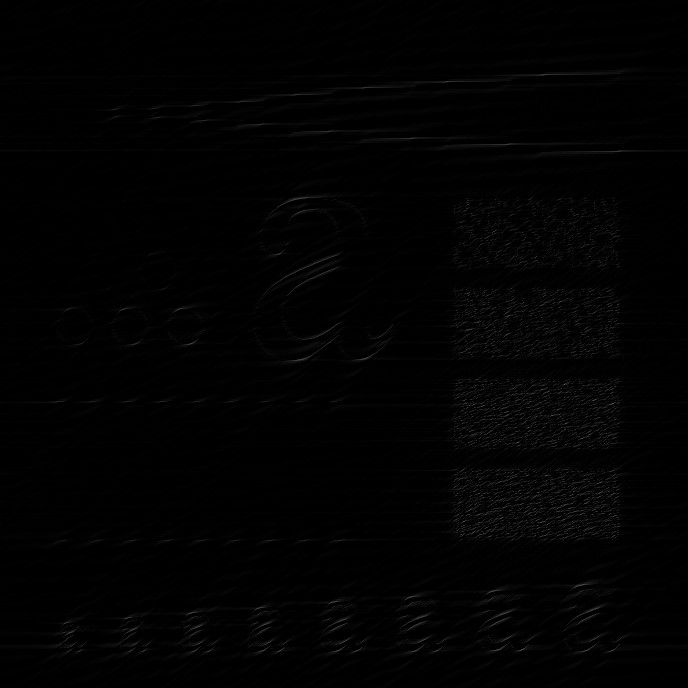
\includegraphics[width=\linewidth]{myfigure/p3/IHPF_1000.png}
		\caption{$D_0=1000$ power ratio=0.0028}
		\label{fig:IHPF_1000}
	\end{subfigure}
  	\caption{Results of ideal highpass filtering.}
  	\label{fig:IHPF}
\end{figure}

\begin{figure}[h!]
	\centering
	\begin{subfigure}[b]{0.3\linewidth}
		
\includegraphics[width=\linewidth]{myfigure/p3/BHPF_10.png}
		\caption{$D_0=10$ power ratio=0.0885}
		\label{fig:BHPF_10}
	\end{subfigure}
  	\begin{subfigure}[b]{0.3\linewidth}
		
\includegraphics[width=\linewidth]{myfigure/p3/BHPF_100.png}
		\caption{$D_0=100$ power ratio=0.0759}
		\label{fig:BHPF_100}
	\end{subfigure}
	\begin{subfigure}[b]{0.3\linewidth}
		
\includegraphics[width=\linewidth]{myfigure/p3/BHPF_1000.png}
		\caption{$D_0=1000$ power ratio=0.0069}
		\label{fig:BHPF_1000}
	\end{subfigure}
  	\caption{Results of Butterworth highpass filtering.}
  	\label{fig:BHPF}
\end{figure}

\begin{figure}[h!]
	\centering
	\begin{subfigure}[b]{0.3\linewidth}
		
\includegraphics[width=\linewidth]{myfigure/p3/GHPF_10.png}
		\caption{$D_0=10$ power ratio=0.0.0873}
		\label{fig:GHPF_10}
	\end{subfigure}
  	\begin{subfigure}[b]{0.3\linewidth}
		
\includegraphics[width=\linewidth]{myfigure/p3/GHPF_100.png}
		\caption{$D_0=100$ power ratio=0.0755}
		\label{fig:GHPF_100}
	\end{subfigure}
	\begin{subfigure}[b]{0.3\linewidth}
		
\includegraphics[width=\linewidth]{myfigure/p3/GHPF_1000.png}
		\caption{$D_0=1000$ power ratio=0.0054}
		\label{fig:GHPF_1000}
	\end{subfigure}
  	\caption{Results of Gaussian highpass filtering.}
  	\label{fig:GHPF}
\end{figure}


\subsection{Discussion}
In lowpass filter smoothing, the larger the $D_0$ is the less blurring there is in the images. In ideal lowpass filtering, we can clearly see ringing in Figure.\ref{fig:ILPF_10} and Figure.\ref{fig:ILPF_100}. This ringing is a characteristic of ideal lowpass. The Fourier transform of a vertical falling is the combination of infinite number of triangle functions. In Butterworth filtering with order $n=2$, there are still mild ringing but much less than those in the ideal filtering. I also notice a little vertical texture in the left part of the result images. In Gaussian lowpass filtering, we hardly see ringing and this is an important benefit in medical image processing because any artifact is unacceptable. However, Gaussian lowpass filtering provide less power ratio than the Butterworth with the same $D_0$. \\

In highpass filter sharpening, the larger the $D_0$ is the darker the result image is. This is because that the remain high frequency component is less when $D_0$ gets large. Thus the highpass result can help us to understand what the so-called high frequency component is in an image. It's not simple to find out differences between Butterworth highpass and Gaussian highpass. However, we can easily see that these two are much sharpen than the result of ideal highpass filtering which is influenced by ringing again.

\subsection{Implementation}
The key part of the implementation is to correctly follow the steps of frequency domain filtering. The steps are encapsulated in function \emph{dft\_filter\_func} in Code.\ref{code:dft_filter_func}. Another thing to talk is how to generate the filter which is implemented in \emph{gen\_filter} in Code.\ref{code:gen_filter}.

\clearpage
\lstset{language=Matlab}
\begin{lstlisting}
function [ imgg, energy_ratio ] = dft_filter_func( imgf, H )
%DFT_FILTER_FUNC 
%   DFT_FILTER_FUNC accept an image imgf, and a filter H
%   output the filtered image imgg and enegy_ratio

% automatically pad imgf: pad_f
imgf = double(imgf);
% fast fourier transform 
F = fft2(imgf);
% filtered by H
G = H .* F;
% inverse fft and obtain the real part
imgg = real(ifft2(G));
% cut out the original size
imgg = uint8(imgg);
% calculate energy ratio
energy_f = sum(sum( abs(F).^2 ));
energy_g = sum(sum( abs(G).^2 ));
energy_ratio = energy_g / energy_f;

end
\end{lstlisting}

\lstset{language=Matlab} 
\begin{lstlisting}
function [ U, V ] = gen_filter( P, Q )
%GEN_FILTER generate filter

u = (0:P-1);
v = (0:Q-1);
idx = find(u > P/2);
u(idx) = u(idx) - P;
idy = find(v > Q/2);
u(idy) = u(idy) - Q;
[V, U] = meshgrid(v, u);

end
\end{lstlisting}

